\problemname{Ski Jumping}

Ski jumping is one of the most popular winter sport competitions.
In the chase of records, ski jumping hills become larger and larger.
To ensure the safety of the competitors, landing speed and angle must not exceed critical margins defined by the FIS.
Today, it's your task to assess these values for a newly constructed ski jumping arena shown in the figure.

\vskip2em
\begin{center}
  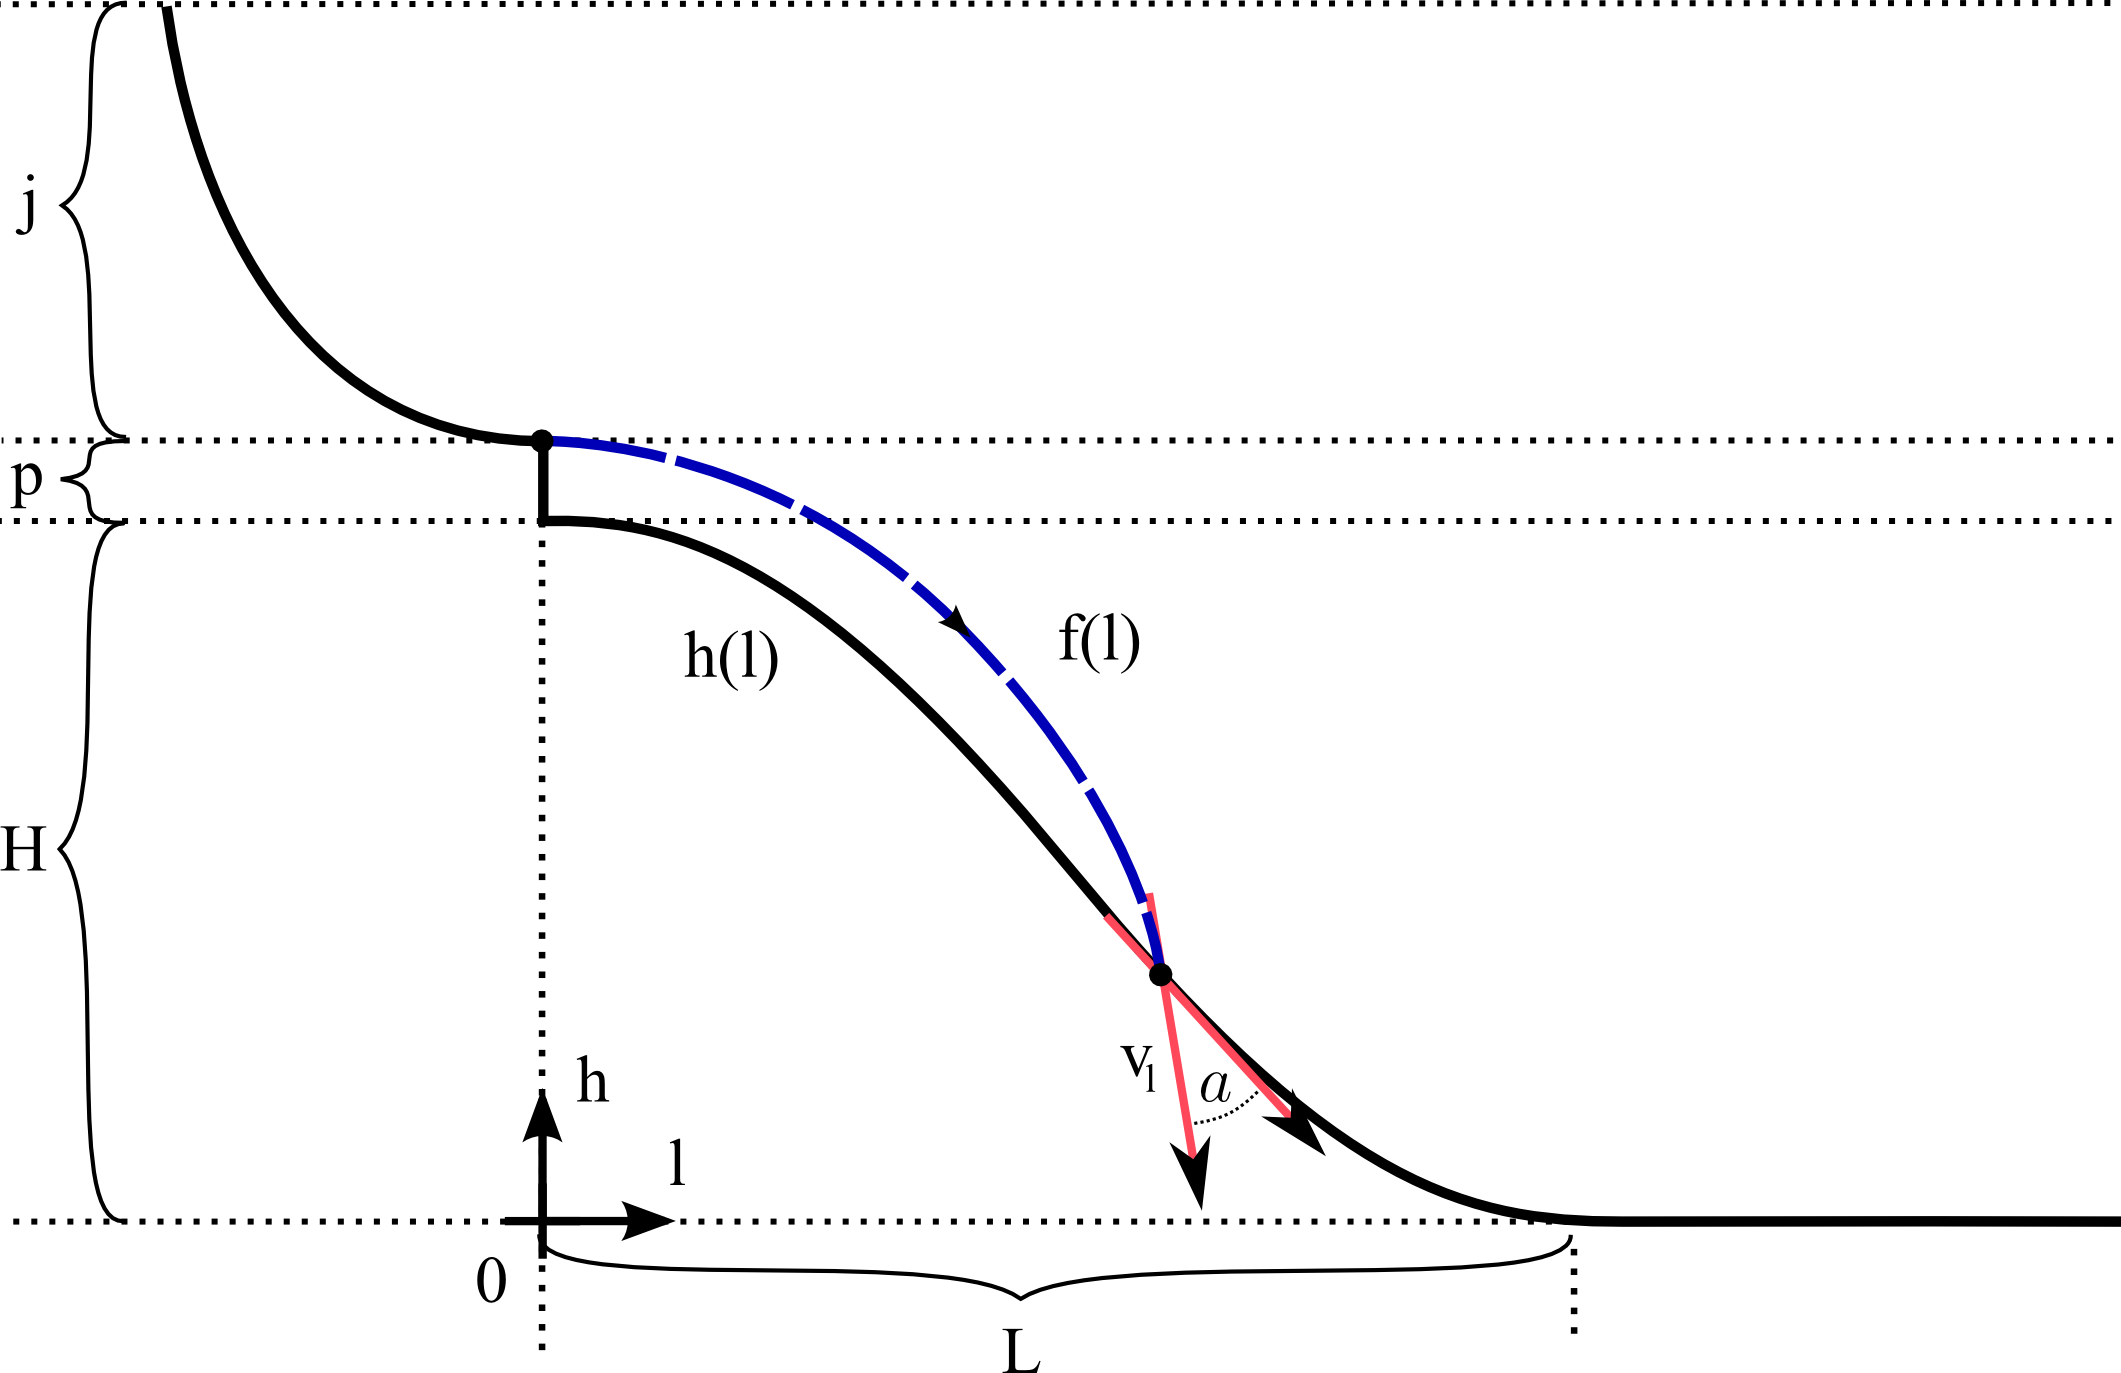
\includegraphics[width=0.9\textwidth]{skijump.png}
\end{center}
\vskip1em

Instead of doing measurements in the field, you can use a little math to solve your problem, since
the hill has the following shape:
\begin{equation}
h(l) = \begin{cases}
   H                                                          &\;\,               l <  0           \\
   H\cdot\left( 1 - 2 \cdot\left(\frac{l}{L}\right)^2 \right) &\; 0           \le l < \frac{L}{2}  \\
  2H\cdot\left( \frac{l}{L} - 1 \right)^2                     &   \frac{L}{2} \le l < L            \\
   0                                                          &\, L           \le l
\end{cases}
\,
\end{equation}
where $l$ is the position on the x-axis with its origin in the beginning of the hill.
$H$ is the height and $L$ is the width of the hill; $j$ is the maximum starting height of the
ski-jump and $p$ is the height difference between the end of the (ski-jump) approach and the top of the hill. 
Assuming that friction plays no important role and since the critical margins are defined for a flight without any
influence of wind, you may utilize the following flight curve:
\begin{equation}
  f(l) = -\frac{g}{2}\cdot\left(\frac{l}{v_0}\right)^2 + H + p
  \qquad \left(\; 0 \le l  \;\wedge\;  f(l) \ge h(l) \;\right)
\,
\end{equation}
where $v_0$ is the speed gained in the approach. You can obtain this value from the law of energy conservation.
Potential and kinetic energy are defined as follows:
\begin{equation}
  E_\mathrm{kin} = \frac{1}{2} \times \mathrm{mass} \times \mathrm{speed}^2
  \,,\qquad
  E_\mathrm{pot} = \mathrm{mass} \times g \times \mathrm{height}
  \,.
\end{equation}
In all equations, $g$ is the gravitational constant ($g\approx9.81\,\mathrm{m\,s}^{-2}$).

\vskip2em
\textbf{Hints:}

The inner product of two vectors $\vec{a}$ and $\vec{b}$ is defined as:
\begin{equation}
  \vec{a}\cdot\vec{b} = |\vec{a}|\cdot|{\vec{b}}|\cdot\cos\measuredangle(\vec{a},\vec{b})
\end{equation}


\section*{Input}
Input starts with the number of test cases $t$ on a single line ($0 < t < 160\,000$).

Every test case consists of a single line containing four positive integers
$j$, $p$, $H$, and $L$ as defined in the problem statement ($0 < j,p,H,L \le
500$). The unit of all values is meter.

\section*{Output}
For every test case, print one line containing
\begin{itemize}
  \item the landing position $l$ on the x-axis,
  \item the landing speed $|v_l|$ of the jumper (in meters per second), and
  \item the speed-angle $\alpha$ (in degree) with respect to the hill (see the figure).
\end{itemize}
The values must be separated by a single blank.
An absolute or relative error of $10^{-4}$ is tolerated.
